\documentclass[hyperref={pdfpagelabels=false}]{beamer}
\usepackage{lmodern}
\usetheme{Antibes}
\title{Come domotizzo casa nonostante mia Moglie}
\subtitle{La domotica col copy and paste}  
\author{Davide Isoardi}
\date{Linx Day Torino - 2022/10/22} 

\newif\ifshowtoc
\showtoctrue% toggles to show the toc
% set captions with numbers
\setbeamertemplate{caption}[numbered]
\AtBeginSection{%
	\ifshowtoc
	\begin{frame}
		\tableofcontents[currentsection, subsectionstyle=show/show/hide]
	\end{frame}
	\fi
}

\hypersetup{
	colorlinks,
	urlcolor=blue
}

\begin{document}
	\begin{frame}
		\titlepage
	\end{frame} 
	
	
	\begin{frame}
		\frametitle{ToC}
		\tableofcontents[hidesubsections]
	\end{frame} 
	
	
	\section{Ci sono io?} 
	\begin{frame}
		\frametitle{Chi sono io?} 
		Sono un nerd (all'antica) che lavora come informatico in una società di consulenza ad alta specializzazione che non ha a che vedere con la domotica.
		
		Quindi la domotica si può capire anche se non è il tuo mestiere
	\end{frame}
	\showtocfalse% toggles to not show the toc
	\section*{Remerciements}
	\begin{frame}
		\begin{block}{Non sono fidelizzato ne sponsorizzato, ma posso fornirvi le mie esperienze e quindi vi dirò nomi e cognomi degli spunti e degli accessori che ho usato - nel bene e nel male}
		\end{block}
	\end{frame}
	\section{Home Assistant}
	\begin{frame}
		\frametitle{Home Assistant}
		\begin{itemize}
			\item E' un hub per la domotica
			\item E' ovviamente open-source
			\item E' locale: non usa il cloud (se vuoi lo usi certo)
			\item Lo sviluppo è basato sulla community oltre al team di sviluppo ufficiale
			\item E' modulare
		\end{itemize}
		\medskip
		\normalsize Qui la home del progetto: \href{https://www.home-assistant.io/}{link}\\	\normalsize Qui i repo: \href{https://github.com/home-assistant}{link}
	\end{frame}
	
	
	\section{Home Assistant} 
	\subsection{Deploy}
	\begin{frame}
		\frametitle{Hardware}
		\begin{itemize}
			\item NUC/Mini PC 
			\item Raspberry PI (3 o 4 - meglio)
			\item Vecchio PC
			\item Proxmox
		\end{itemize}
	\end{frame}

	\begin{frame}
		\frametitle{Modalità di deploy}
		\begin{itemize}
			\item Home Assistant OS  
			\item Home Assistant Supervised su Docker 
			\item Home Assistant Core 
			\item Home Assistant Core su Docker
		\end{itemize}
	\medskip
		\normalsize Per iniziare vi consiglio di documentarvi su indomus.it e in particolare da questa pagina: \href{https://indomus.it/formazione/home-assistant-su-raspberry-pi-varie-installazioni-le-cose-da-fare/}{link}
	\end{frame}
	
	\begin{frame}
		\frametitle{Il mio deploy}
		\begin{itemize}
			\item Rpi4 (4GB RAM)  
			\item Docker ma con supervisor
		\end{itemize}
		\begin{figure}
			\centering
			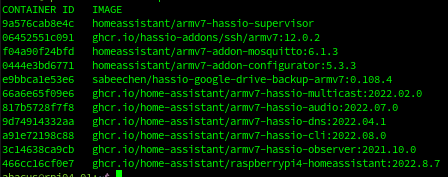
\includegraphics[width=0.75\textwidth]{./images/docker-ps.png}
			\caption{docker ps}
			\label{fig:docker-ps}
		\end{figure}
	\end{frame}
	
	\section{Integrazioni}
	\begin{frame}
		\frametitle{Integrazioni}
		\begin{itemize}
			\item Native  
			\item HACS - \href{https://hacs.xyz}{link}
			\item Add-on
		\end{itemize}
		\begin{block}{Alcune integrazioni, tipo quella ufficiale con Alexa, sono abilitabili tramite il servizio cloud di Nabu casa (\href{https://www.nabucasa.com/}{link}) che permette di esporre il tuo home assistant anche al di fuori della rete domestica}
		\end{block}
	\end{frame}

	\subsection{Native}
	\begin{frame}
	\frametitle{Native}
		\href{https://www.home-assistant.io/integrations}{Qui}
		una lista completa di quelle presenti. Considerate che se ne aggiungono ad ogni release.
		\begin{figure}
			\centering
			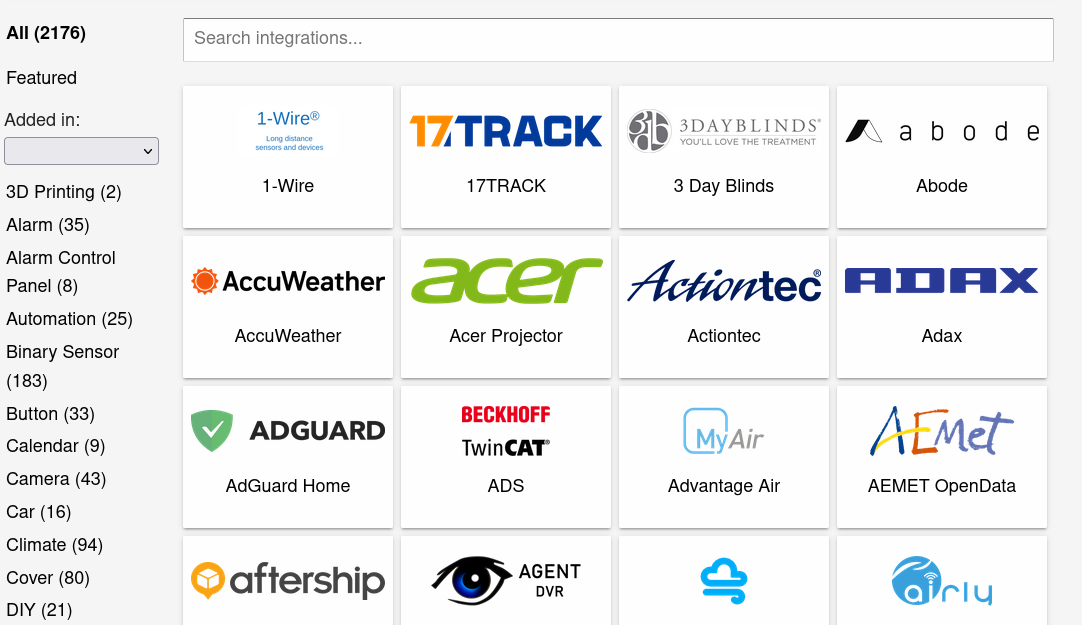
\includegraphics[width=0.75\textwidth]{./images/core-integrations.png}
			\caption{Integrazioni native}
			\label{fig:core-integration}
		\end{figure}
	\end{frame}

	\subsection{HACS}
	\begin{frame}
	\frametitle{HACS}
	\normalsize E' il Home Assistant Community Store - si divide in:
	\begin{itemize}
		\item integrazioni - altre integrazioni ma gestite dalla community
		\item frontend - componenti aggiuntive per le dashboard
	\end{itemize}
	\begin{figure}
		\centering
		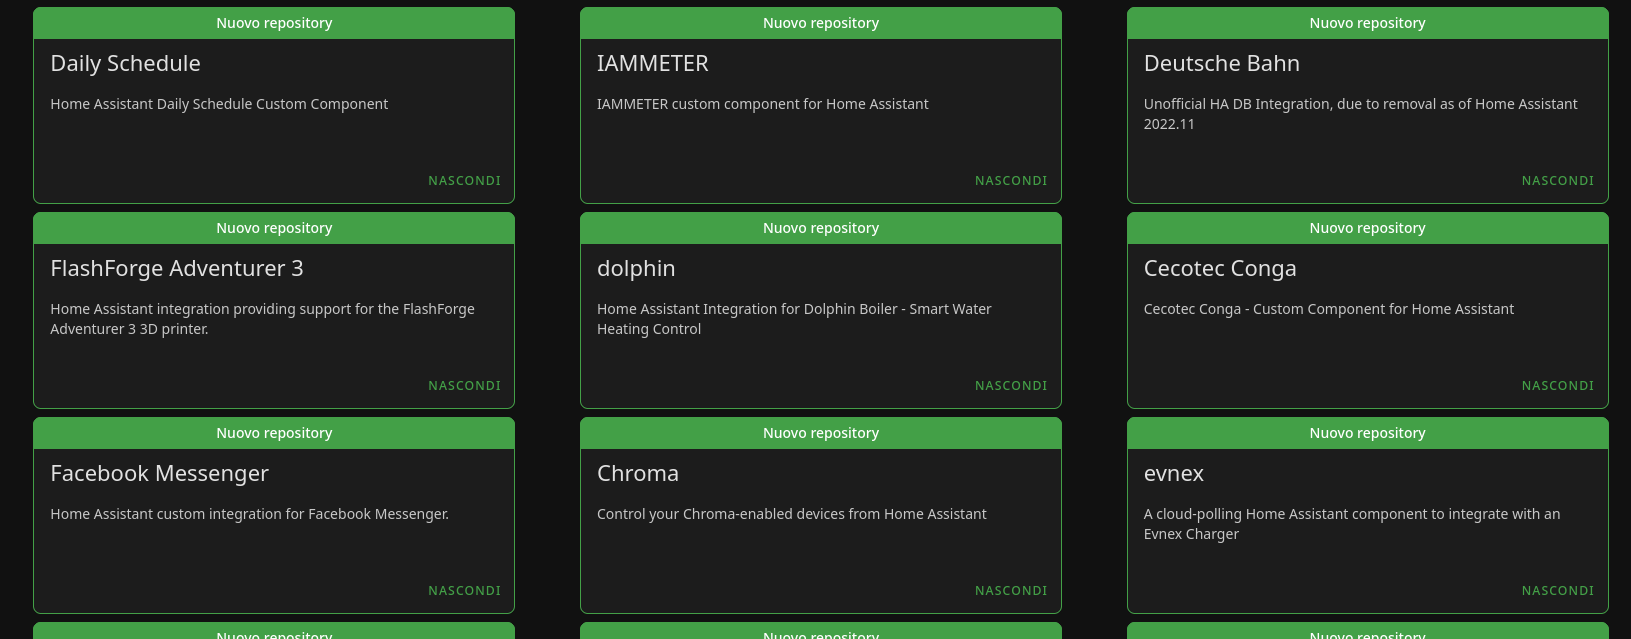
\includegraphics[width=0.4\textwidth]{./images/hacs-integrations.png}\quad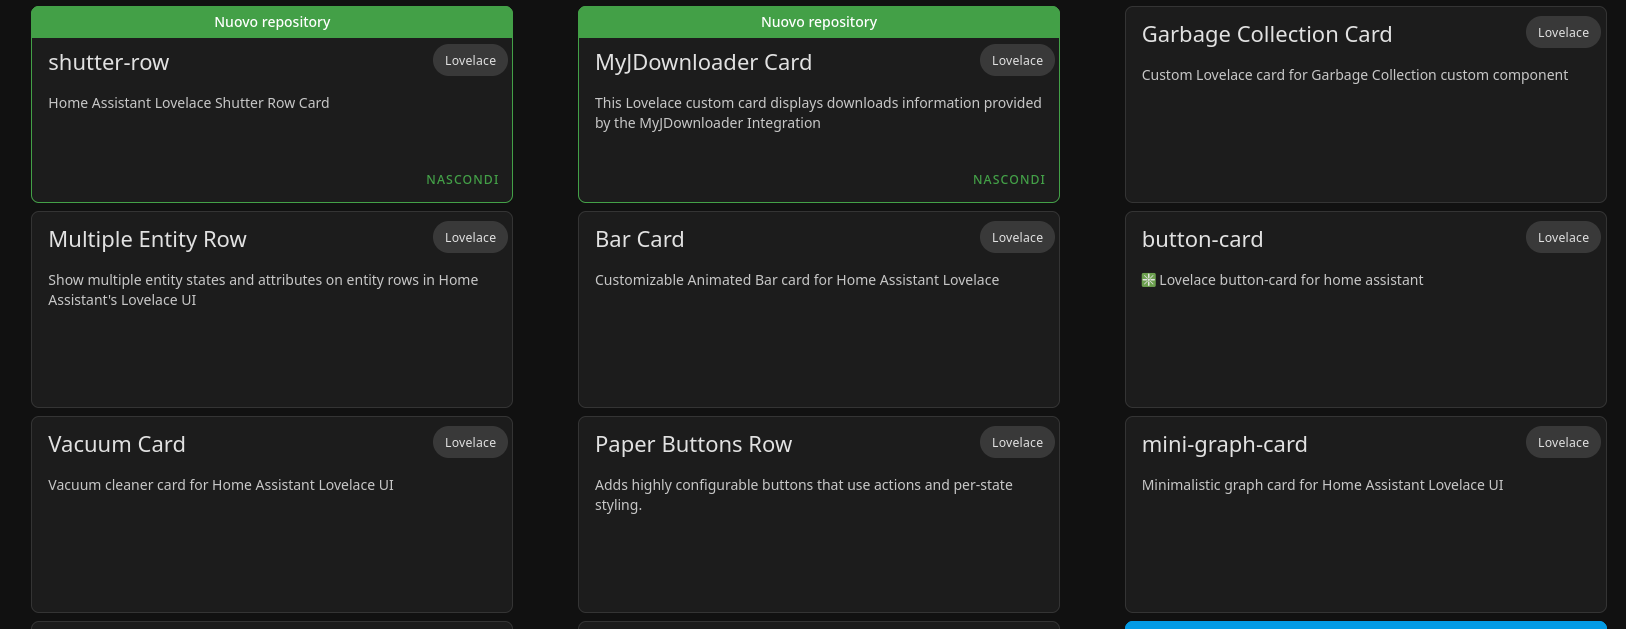
\includegraphics[width=0.4\textwidth]{./images/hacs-frontend.png}
		\caption{HACS}
		\label{fig:hacs-integration}
	\end{figure}
	\end{frame}

	\subsection{Add-on}
	\begin{frame}
	\frametitle{Add-on}
	\normalsize Direi che è autoesplicativo. Aggiungo solo che è possibile aggiunre nuovi add-on semplicemente trovandoli su internet e inserendo il repo git.
	\begin{figure}
		\centering
		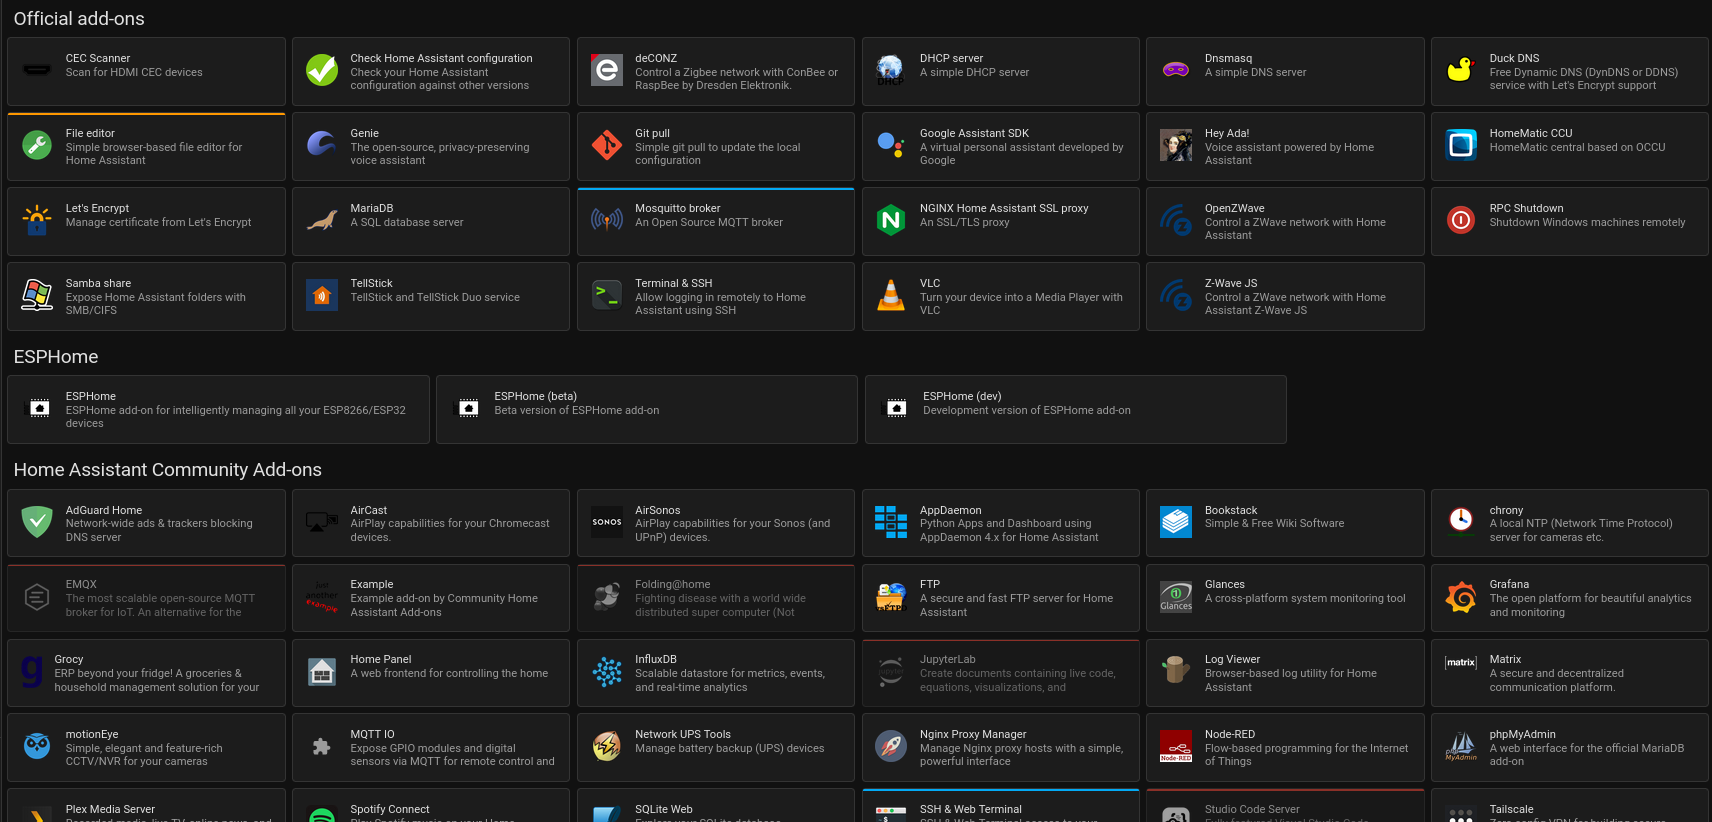
\includegraphics[width=0.75\textwidth]{./images/add-on.png}
		\caption{Add-on}
		\label{fig:add-on}
	\end{figure}
	\end{frame}

	\section{Casa Mia}
	\begin{frame}
	\frametitle{Cosa uso}
	\begin{itemize}
		\item RaspberryPI 4 con 4 core e 4GB di RAM (no external device)
		\item Installazione Docker con supervisor
		\item IoT prevalentemente shelly -  \href{https://shelly.cloud/}{Official site}
		\item Google Drive per il backup
		\item Nabu casa per accesso esterno e per Alexa
		\item Home assistant companion
	\end{itemize}
	\end{frame}

	\begin{frame}
	\frametitle{Cosa faccio}
	\begin{itemize}
		\item Automazione Lavatrice - Asciugatrice
		\item Automazioni in merito alla presenza in casa - fuori casa
		\item Controllo consumi
		\item Gestione termica
		\begin{itemize}
			\item Riscaldamento sopra/sotto
			\item Pompe di calore
			\item Tende esterne
			\item Controllo calendario
		\end{itemize}
		\item Irrigazione
	\end{itemize}
	\end{frame}

	\begin{frame}
	\frametitle{La ToDo list}
	\begin{itemize}
		\item Riscaldamento per stanza (sopra)
		\item Controllo consumi stanze mancanti
		\item Irrigazione con controllo meteo e stato prato
		\item Ciclo di risveglio
	\end{itemize}
	\end{frame}

	\section{Appendice}
	\begin{frame}
	\frametitle{Ringraziamenti}
	\begin{itemize}
		\item Gruppo facebook  Home Assistant Italia - \href{https://www.facebook.com/groups/147299622598134}{Link}
		\item inDomus - \href{https://indomus.it/}{Link}
		\item hassioHelp - \href{https://hassiohelp.eu/}{Link}
		\item Max Albani - \href{https://www.maxalbani.it/}{Link}
		\item Salvatore Lentini e DomHouse - \href{https://domhouse.it/}{Link}
	\end{itemize}
\end{frame}
\end{document}
